\section*{Mini Machine Problem 1 (15 points)}
This MP borrows a quite considerable amount of material from a certain source. We will publish the source after the submission’s due date because it contains answers for a few questions. Don’t try to find the existing answers because the MP is not hard, and it is really fun and useful. To finish the MP, please read this document carefully.\\
In this MP, we use the Matlab  built-in data set \textbf{carsmall}, a data set containing information for 100 cars in 1970, 1976 and 1982. For this data set, we focus on 5 attributes: \texttt{Acceleration} (the rate of change of velocity of a car), \texttt{MPG} (Miles Per Gallon, fuel efficiency), \texttt{Displacement} (the volume of the cylinder), \texttt{Horsepower} and \texttt{Weight}. We use the \texttt{Cylinders} attribute (the number of cylinders) to group our observation. You will be required to run some code provided to you in this PDF file. \textbf{However, do not copy the code from this file to Matlab directly since the encoding mechanism for some special symbol in PDF is not supported by Matlab. You should type the code into Matlab.}\\

\textbf{Purpose} 
\begin{itemize}
\item Learn the basic techniques for data visualization using Matlab.
\end{itemize}
\textbf{Requirements} 
\begin{itemize}
\item This MP requires Matlab. \textit{Please do not use other softwares since that will make the assignment harder for some questions.} The software is free for UIUC students in UIUC Webstore. And it is also available in EWS machines on campus. If you are not able to access both sources, please let us know ASAP. Please also note that it may take you only 1-2 hours to finish the MP, so if you don’t often use the heavy Matlab software, you may want to use one of the EWS machines on campus.
\item You should write all your answers (code, graphs and texts) in the PDF file you will submit. For code and graphs, you could paste them to the file.  
\end{itemize}
 

\begin{enumerate}
\item[1.] Load the data \textbf{carsmall} in Matlab using the following code.
\begin{lstlisting}
load carsmall
X = [MPG,Acceleration,Displacement,Weight,Horsepower];
varNames = {'MPG'; 'Acceleration'; 'Displacement'; 'Weight'; 'Horsepower'};
\end{lstlisting}
\item[2.] (2') Comet graph is an animated graph. To trace the data points on the screen for the \texttt{Displacement} attribute, we use the following code to visualize the \texttt{Displacement} attribute. Show the \textbf{final comet graph} in the PDF file you will submit by running the following code on Matlab.
\begin{lstlisting}
comet(Displacement)
xlabel('Index of Car')
ylabel('Displacement')
\end{lstlisting}

\item[3.] (5') Drawing boxlpot is a popular way to visualize a distribution. The two whiskers show the Min observation and the Max observation. The central line shows the median. The edges of the box are the first quantile and the third quantile. 
\begin{itemize}
\item[a.] (1') Run the following code on your Matlab to draw a boxplot for the \texttt{Acceleration} attribute. Show the \textbf{boxplot}  in the PDF file you will submit.
\begin{lstlisting}
boxplot(Acceleration)
ylabel('Acceleration')
\end{lstlisting}
\item[b.] (4') Write code to visualize the \texttt{Acceleration} attribute using the boxplot for cars with different number of cylinders. In this graph, you group cars using the \texttt{Cylinders} attribute (the number of cylinders). For each group of cars, you draw a box to show the five-number summaries on \texttt{Acceleration}.  All the boxes should be drawn on the same graph. In your graph, $x$-axis represents the number of cylinders and the $y$-axis shows the \texttt{Acceleration}. You should also add the label for $x$-axis (\texttt{Cylinders}) and $y$-axis (\texttt{Acceleration}). (\textit{Hint: only several lines of codes are needed to finish this task. Try to use the boxplot(X,G) function where X is the attribute to be visualized and G is the grouping attribute.})
Show your \textbf{code and grouping boxplot} in the PDF file you will submit. 
\end{itemize}

\item[4.] (4') 3-D scatter plots are popularly used to visualize 3 attributes at the same time. 
\begin{itemize}
\item[a.] (2') Run the following code to draw a 3-D scatter plot. Show the \textbf{3-D plot} in the PDF file you will submit. 
\begin{lstlisting}
scatter3(Displacement,Cylinders,Horsepower,'filled','r')
xlabel('Displacement')
ylabel('Cylinders')
zlabel('Horsepower')
\end{lstlisting}
\item[b.] (2') By observing the graph you get, could you identify a pair of correlated attributes? Could you explain why the positive or negative correlation makes sense? Give your \textbf{answer} in the PDF file you will submit. (\textit{Hint: You could rotate the graph in Matlab when you try to find the correlation between two attributes on a 3-D graph.})
\end{itemize}

\item[5.] (4') Interactive star plots are used to show the values of attributes for each observation. In each star (observation), the spoke length is proportional to the value of that attribute for that observation.
\begin{itemize}
\item[a.] (2') Run the following code. Show the \textbf{graph} in PDF file you will submit.
\begin{lstlisting}
h = glyphplot(X(1:9,:), 'glyph','star', 'varLabels',varNames,...
'obslabels',Model(1:9,:));
set(h(:,3),'FontSize',8);
\end{lstlisting}
\item[b.] (2') In the Matlab figure dialog menu, there is a button called \textbf{data cursor} (See Figure \ref{fig:datacuror}. The data cursor item is in the red circle.) Based on the graph you get in 5a, if you click on the data cursor button, and then click on any star (car), you will get the value for each attribute of that car. Show the \textbf{value} of each attribute for the star (car) at the top left corner of the graph you plotted in the Question 5a in the PDF file you will submit.
\begin{figure}[!h]
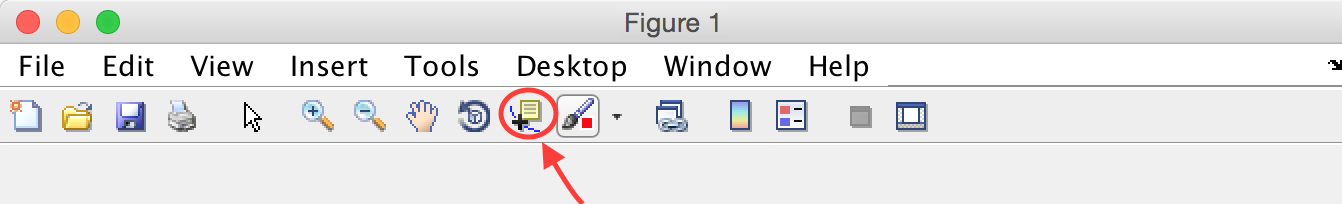
\includegraphics[width=0.5\textwidth]{pics/datacursor.png}
\centering
\caption{Matlab Figure Dialog Menu}
\label{fig:datacuror}
\end{figure}
\end{itemize}

\end{enumerate}